\documentclass[tikz,border=10pt]{standalone}
\usepackage{tikz,amsmath}
\usetikzlibrary{shapes.geometric, positioning, arrows.meta,calc,fit}

\begin{document}
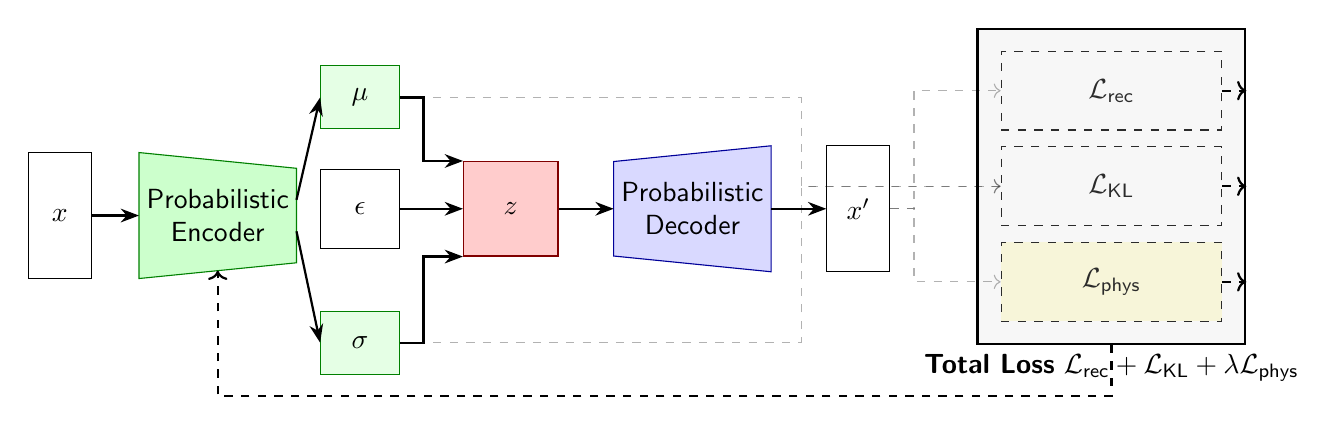
\begin{tikzpicture}[
  font=\sffamily, 
  node distance=1.2cm and 1.4cm, 
  arrow/.style={->, thick, >=Stealth},
  encoder/.style={draw=green!50!black, fill=green!20, minimum height=1.6cm},
  decoder/.style={draw=blue!60!black, fill=blue!15, minimum height=1.6cm},
  box/.style={draw, minimum width=0.8cm, minimum height=1.6cm},
  smallbox/.style={draw=green!50!black, fill=green!10, minimum width=1cm, minimum height=0.8cm},
  epsbox/.style={draw, minimum width=1.0cm, minimum height=1.0cm},
  latent/.style={draw=red!50!black, fill=red!20, minimum width=1.2cm, minimum height=1.2cm}
]

% Input
\node[box] (x) {$x$};

% Encoder trapezoid
\coordinate[right=0.6cm of x] (enc-left);
\coordinate[right=2cm of enc-left] (enc-right);
\path[draw=green!50!black, fill=green!20] 
  ($(enc-left)+(0,0.8)$) -- 
  ($(enc-right)+(0,0.6)$) --
  ($(enc-right)-(0,0.6)$) --
  ($(enc-left)-(0,0.8)$) -- cycle;
\node[align=center] at ($(enc-left)!0.5!(enc-right)$) {Probabilistic\\Encoder};

% μ and σ vertically aligned
\node[smallbox, right=0.3cm of enc-right, yshift=1.5cm] (mu) {$\mu$};
\node[smallbox, below=2.3cm of mu] (sigma) {$\sigma$};

% ε
% \node[epsbox, right=0.7cm of mu.center, xshift=0.125cm,yshift=-0.55cm] (eps) {$\epsilon$};
\node[epsbox, below=0.5 of mu] (eps) {$\epsilon$};%

% z
\node[latent, right=0.8cm of eps] (z) {$z$};

% Decoder trapezoid
\coordinate[right=0.7cm of z] (dec-left);
\coordinate[right=2cm of dec-left] (dec-right);
\path[draw=blue!60!black, fill=blue!15] 
  ($(dec-left)+(0,0.6)$) -- 
  ($(dec-right)+(0,0.8)$) --
  ($(dec-right)-(0,0.8)$) --
  ($(dec-left)-(0,0.6)$) -- cycle;
\node[align=center] at ($(dec-left)!0.5!(dec-right)$) {Probabilistic\\Decoder};

% Output
\node[box, right=0.7cm of dec-right] (xprime) {$x'$};

% \node[draw, dashed, minimum width=2.4cm, minimum height=1cm, below=of xprime] (physloss) {Physics Loss};
% \draw[->, dashed] (physloss.west) to[bend left=20] node[below] {\footnotesize loss signal} (enc-left);

% Arrows
\draw[arrow] (x) -- (enc-left);
\draw[arrow] ($(enc-right)+(0,0.2)$) -- (mu.west);
\draw[arrow] ($(enc-right)-(0,0.2)$) -- (sigma.west);
\draw[arrow] (mu.east) -- ++(0.3,0) |- (z.north west);
\draw[arrow] (sigma.east) -- ++(0.3,0) |- (z.south west);
\draw[arrow] (eps.east) -- (z.west);
\draw[arrow] (z.east) -- (dec-left);
\draw[arrow] (dec-right) -- (xprime);


% Orthogonal curved loop from Physics Loss to Encoder
% Orthogonal loop from Physics Loss to bottom of Encoder
% \draw[->, dashed, thick] 
%   (physloss.west) -- ++(-8.3,0) 
%   |- ($(enc-left)-(0,0.8)$);  % targets bottom of encoder

% % Optional: loss gradient label near bottom path
% \node[font=\footnotesize, align=center] 
%   at ($(physloss.west)!0.5!($(enc-left)-(0,0.8)$)$) 
%   [yshift=-0.55cm] {loss gradient};

% === Loss Components ===

% Loss boxes aligned vertically to the right of xprime
\node[draw, dashed, minimum width=2.8cm, minimum height=1cm, right=1.4cm of xprime, yshift=1.5cm] (recloss) {$\mathcal{L}_{\text{rec}}$};
\node[draw, dashed, minimum width=2.8cm, minimum height=1cm, below=0.2cm of recloss] (klloss) {$\mathcal{L}_{\text{KL}}$};
\node[draw, dashed, fill=yellow!15, minimum width=2.8cm, minimum height=1cm, below=0.2cm of klloss] (physloss) {$\mathcal{L}_{\text{phys}}$};

% \draw[->, dashed] (xprime.south) -- ++(0,-.05) -| (physloss.west);


% Total Loss Box wrapping them
\node[draw=black,fill=black!15, fill opacity=0.2, thick, minimum width=3.4cm, minimum height=4cm, fit=(recloss)(physloss), label=below:{\textbf{Total Loss} $\mathcal{L}_{\text{rec}} + \mathcal{L}_{\text{KL}} + \lambda \mathcal{L}_{\text{phys}}$}] (totallosspanel) {};

% Backpropagation arrow from Total Loss box to Encoder
\draw[->, dashed, thick] 
  (totallosspanel.south) 
   -- ++(0,-.65) -| 
  ($(enc-left)-(-1,0.7)$);


% Arrows showing where each loss comes from

% L_rec from x and x'
% \draw[->, dashed, opacity=0.3] (x.south) -- ++(0,-0.6) -| (recloss.west);
\draw[->, dashed, opacity=0.3] (xprime.east) -- ++(0.3,0) |- (recloss.west);

% L_KL from mu and sigma
\draw[->, dashed, opacity=0.3] (mu.east) -- ++(5.1,0) |- (klloss.west);
\draw[->, dashed, opacity=0.3] (sigma.east) -- ++(5.1,0) |- (klloss.west);

% L_phys from x'
\draw[->, dashed, opacity=0.3] (xprime.east) -- ++(0.3,0) |- (physloss.west);

% From each loss to total loss box
\draw[->, dashed, thick] (recloss.east) -- (totallosspanel.east |- recloss.east);
\draw[->, dashed, thick] (klloss.east) -- (totallosspanel.east |- klloss.east);
\draw[->, dashed, thick] (physloss.east) -- (totallosspanel.east |- physloss.east);

\end{tikzpicture}
\end{document}
